\documentclass{beamer}
\mode<presentation>
\usetheme{CambridgeUS}
\usepackage[russian]{babel}
\usepackage[utf8]{inputenc}
\usepackage[T2A]{fontenc}
\usepackage{sansmathaccent}
\pdfmapfile{+sansmathaccent.map}
\title{Фильтрация}
\author{Наумов Д.А.}
\date[19.03.2014] {Компьютерные музыкальные технологии и звуковой дизайн, 2014}

\begin{document}

%ТИТУЛЬНЫЙ СЛАЙД
\begin{frame}
  \titlepage
\end{frame}

%СОДЕРЖАНИЕ ЛЕКЦИИ
\begin{frame}
  \frametitle{Содержание лекции}
  \tableofcontents
\end{frame}

%РАЗДЕЛ 1
\section{Частотные диапазоны}
\begin{frame}
Перед тем как приступать к частотной коррекции звука, необходимо знать, какая звуковая информация содержится в различных частях спектра. Рассмотрим это на следующем примере: треки \emph{track01-track09} являются версиями одного и того же трека.

Каждый трек содержит:
\begin{itemize}
\item мужскую речь;
\item женскую речь;
\item электронную музыку;
\item запись оркестра;
\item песню в стиле pop-music, исполняемую женщиной;
\item хард-рок c мужским вокалом.
\end{itemize}

Звук в файле  \emph{track01} записан с полным качеством. Другие треки обработаны с помощью фильтров, при помощи которых из исходного трека были удалены частотные составляющие, не входящие в определенный частотный диапазон.
\end{frame}

\begin{frame}
Традиционно, весь звуковой диапазон условно разделяется на:
\begin{itemize}
\item низкие~--- до 200~Гц;
\item средние~--- от 200~Гц до 5000~Гц;
\item высокие~--- от 5~000~Гц до 20~000~Гц.
\end{itemize}
Выбор частот в следующих примерах не является рекомендацией для выполнения коррекции спектра, а предназначен лишь для ознакомления со звуковыми диапазонами.
\end{frame}

\subsection{Диапазон $10..100$~Гц}
\begin{frame}
Это самые низкие звуки, которые воспринимает наш слух. Если звуковоспроизводящая аппаратура не воспроизводит эти частоты, то будет ощущаться потеря насыщенности и глубины звука. Однако, большая часть данного диапазона специально отфильтровывается при записи речи, чтобы избежать низкочастотного гула. 

В записи \emph{track02} первые четыре секунды тишины являются женским голосом~--- звука не слышно, так как в женском голосе почти нет энергии в этом диапазоне. Очень мало мужского голоса в следующих четырех секундах. Электронная и оркестровая музыка является скудной, присутствуют только случайные ноты.

\centering{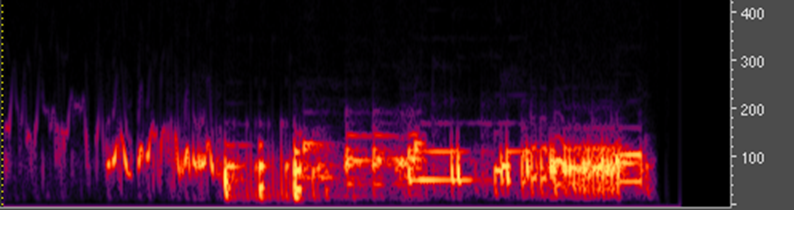
\includegraphics[width=0.75\textwidth]{pic-specter-01}}
\end{frame}

\subsection{Диапазон $100..300$~Гц}
\begin{frame}
Этот диапазон содержит верхние ноты басовых инструментов, основные гармоники таких инструментов, как гитара и основные гармоники речи. Если потерять этот регистр, то вместе с ним потеряется и ощущение силы звука, так как в этих частотах содержится энергия звука, которая заставляет вас пританцовывать под музыку, недаром основная энергия ритм-секции сконцентрирована именно в этом регистре.

Прослушивая \emph{track03}, обратите внимание, что мужской и женский голос имеют здесь почти одинаковую энергию. Однако, разобрать гласные звуки невозможно. При записи вокала и речи гармоники в этом диапазоне будут маскироваться инструментами, и вы их вряд ли услышите.

\centering{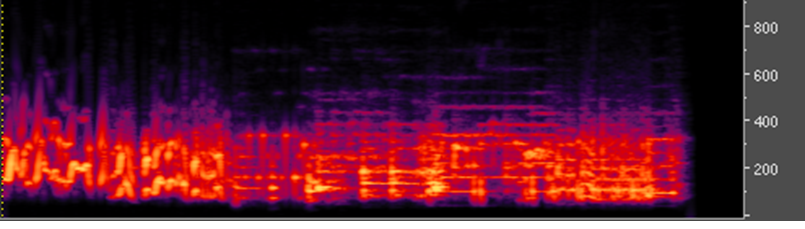
\includegraphics[width=0.75\textwidth]{pic-specter-02}}
\end{frame}

\subsection{Диапазон $300..600$~Гц}
\begin{frame}
Этот диапазон содержит нижние гармоники для частот речи и практически весь аккомпанемент. Хотя это первый диапазон, в котором мы можем различить гласные звуки, для различимости речи он не так важен. Тем не менее этот и следующий диапазоны содержат большую часть энергии человеческого голоса.

Так как этот диапазон содержит основную и верхние гармоники большинства мелодических инструментов, есть вероятность того, что при сведении голос и музыка будут состязаться между собой. Прослушивая \emph{track04}, можно услышать, как инструменты, задающие мелодию, отступают, когда начинается пение. 

\centering{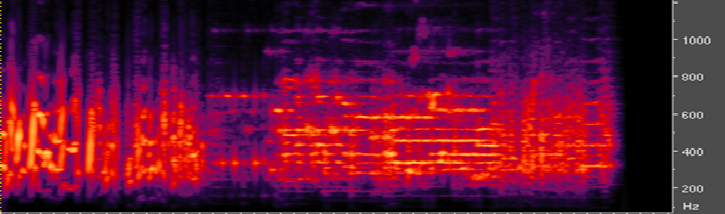
\includegraphics[width=0.75\textwidth]{pic-specter-03}}
\end{frame}

\subsection{Диапазон $600..1200$~Гц}
\begin{frame}
Данный диапазон содержит гармоники высшего порядка для основных речевых частот. Прослушивая \emph{track05}, обратите внимание, насколько женский голос, яркий по природе, сильнее в этом диапазоне. Но ни женский, ни мужской голоса не различимы полностью, так как глухие согласные звуки начинаются только в следующей октаве.

Этот диапазон важен для инструментов:первая и вторая гармоники помогают вам различать инструменты. Большинство инструментов имеют здесь значительную энергию. Как правило, в этом диапазоне присутствует соло скрипок, соло гитар, фортепиано. Музыку, в которой не хватает этих частот обычно называют "<занудной"> или "<смурной">.

Cлух человека здесь очень чувствителен к тонким различиям в звучании.

\centering{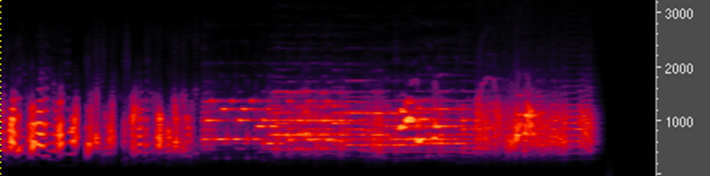
\includegraphics[width=0.75\textwidth]{pic-specter-04}}
\end{frame}


\subsection{Диапазон $1200..2400$~Гц}
\begin{frame}
Этот диапазон важен для речи: здесь у гармоник находится достаточно энергии для того, чтобы различить большинство гласных звуков и все согласные звуки. Диапазон также важен для медных инструментов, имеющих сильные верхние гармоники.

Пение также сильно представлено в этом диапазоне. Но, несмотря на всю активность в этом диапазоне, громкость в \emph{track06} не столь высока. 

\centering{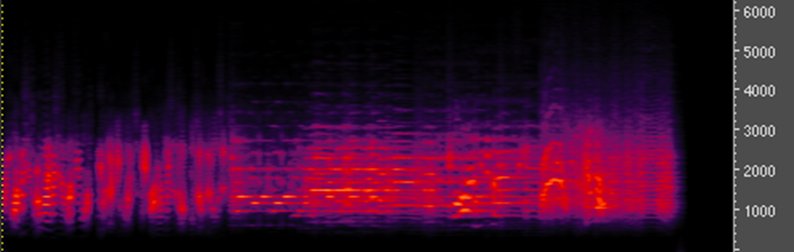
\includegraphics[width=0.75\textwidth]{pic-specter-05}}
\end{frame}

\subsection{Диапазон $2400..4800$~Гц}
\begin{frame}
Хотя большинство гласных звуков и здесь имеют заметные гармоники, но они не важны для различимости речи. Также мало остается от электронной музыки. Здесь сильна оркестровая медь. Большинство медных инструментов очень богаты верхними гармониками, и именно это помогает нам отличать один медный инструмент от другого. Женский вокал основном заглушает струнные в этом частотном диапазоне. Рок-композиция продолжает звучать громко, что типично для танцевальной и рок-музыки.

\centering{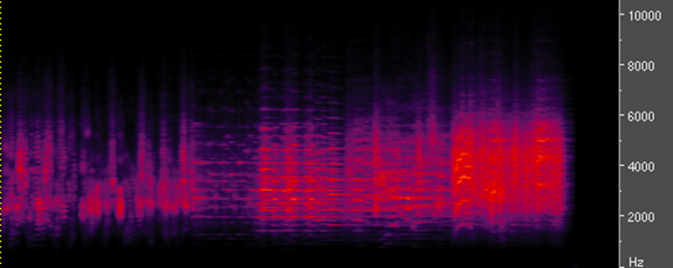
\includegraphics[width=0.75\textwidth]{pic-specter-06}}
\end{frame}

\subsection{Диапазон $4800..9600$~Гц}
\begin{frame}
В этом диапазоне встречается самое сильное искажением высоких частот, шипение пленки в этом диапазоне (для любителей кассетной записи) становится самым заметным, так как здесь очень мало других звуков, способных скрыть это. Хотя люди теоретически могут слышать и более высокие тона, эти частоты считаются пределом восприятия. В треке \emph{track07} вы можете слышать совсем немного женского голоса. От мужского голоса остались лишь согласные звуки. Синтезатор почти полностью исчез. Но медь все еще осталась сильной. Кажется, единственной вещью, сохранившей силу в двух песнях, являются верхние гармоники струнных, вопль гитары и ударные. Громкие звуки отстоят друг от друга значительно дальше, чем в более низких октавах.

\centering{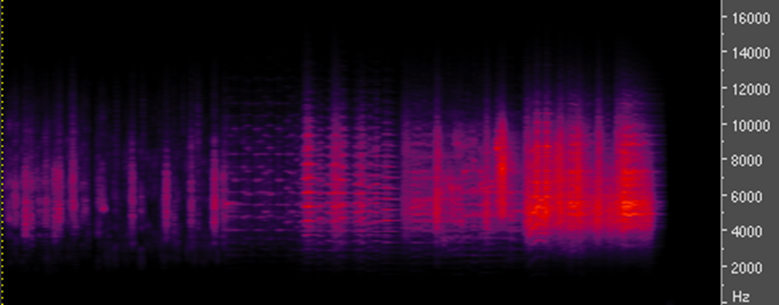
\includegraphics[width=0.75\textwidth]{pic-specter-07}}
\end{frame}

\subsection{Диапазон $9600..20000$~Гц}
\begin{frame}
Это диапазон верхних звуковых частот, верхняя октава всего частотного диапазона, самые "<тонкие"> и "<нежные"> частоты. Если этот диапазон частот будет неполноценен, то вы ощутите некий дискомфорт при прослушивании записей.

В течение почти всего трека \emph{track08} вы можете ничего не слышать. На этих частотах осталось немного оркестровой меди, но от поп-музыки осталось главным образом неразличимое шипение.

\centering{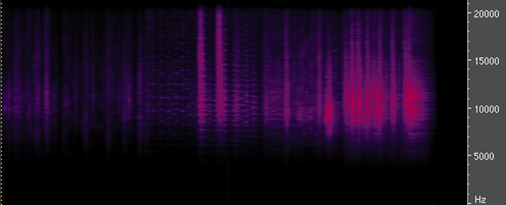
\includegraphics[width=0.75\textwidth]{pic-specter-08}}
\end{frame}

\section{Частотные преобразования сигнала}
\begin{frame}
К преобразованию звука прибегают в основном с целью изменения каких-то его характеристик. Кроме того, на основе описанных ниже преобразований базируются механизмы создания различных звуковых эффектов, а также способы очистки звука от нежелательных шумов, изменения тембра и т.п. Все эти преобразования сводятся, в конечном счете, к следующим:
\begin{itemize}
  \item \emph{Амплитудные преобразования} выполняются над амплитудой сигнала. Такую процедуру можно проделать двумя способами: либо умножая амплитуду сигнала на некоторое фиксированное число, в результате чего получится одинаковое изменение интенсивности сигнала на всей его протяженности, то есть усиление или ослабление, либо изменяя амплитуду сигнала по какому-то закону, то есть умножая амплитуду сигнала на модулирующую функцию. Последний процесс называется \emph{амплитудной модуляцией}.
\end{itemize}
\end{frame}
\begin{frame}
\begin{itemize}      
  \item \emph{Частотные преобразования} выполняются над частотными составляющими звука. Фактически сигнал представляется рядом Фурье, затем производится обработка необходимых частотных составляющих (например, фильтрация) и обратная свертка. В отличие от амплитудных преобразований, эта процедура значительно более сложная в исполнении, так как сам процесс разложения звука на простейшие синусоидальные колебания трудоемок.
  \item \emph{Фазовые преобразования} выполняются либо путем постоянного сдвига фазы сигнала, либо путем наложения некоторой фазомодулирующей функции. Такие преобразования, например, стерео сигнала, позволяют реализовать эффект вращения или "<объёмности"> звука.
  \item \emph{Временные преобразования} реализуются путем наложения на сигнал одной или нескольких его копий, сдвинутых во времени. Позволяют создать эффекты эха или хора. Кроме того, временные преобразования могут влиять на пространственные характеристики звука.
\end{itemize}
\end{frame}

\begin{frame}
\emph{Частотные преобразования} (\emph{частотная коррекция})~--– процесс обработки звукового сигнала с целью изменения его спектрального состава (тембра).
Задачами такой обработки могут быть:
\begin{itemize}
  \item амплитудно-частотная коррекция сигнала;
  \item полное подавление спектра сигнала или шумов в определенной полосе частот;
  \item улучшение разборчивости речи;
  \item легкое изменения характера звука;
  \item подчеркивание басового ритма в музыкальном фрагменте;
  \item имитация телефонов, интеркомов и других реальных громкоговорящих устройств;
  \item компенсация недостатков системы воспроизведения.
\end{itemize}
\end{frame}

\begin{frame}
Есть определенные задачи, которые не могут быть решены при помощи фильтрации:
\begin{itemize}
  \item нельзя удалить случайные и непериодические шумы;
  \item нельзя исправить искаженные записи;
  \item нельзя создать звуки, которых раньше не было в записи (высокие частоты, которые были потеряны при низкочастотной дискретизации или басы, которые были раннее отфильтрованы);
  \item нельзя выделить голос из толпы или исключить солиста или инструменты в оркестре.
\end{itemize}
\end{frame}

\begin{frame}
Основным инструментом частотной коррекции являются \emph{фильтры} и инструменты, созданные на основе фильтров. Фильтр описывается \emph{амплитудно-частотными} (АЧХ) и \emph{фазо-частотными характеристиками} (ФЧХ).

~

\emph{АЧХ}~--- зависимость коэффициента передачи фильтра от частоты. Участок АЧХ, где коэффициент передачи не равен нулю, соответствует полосе пропускания фильтра. В полосе задерживания (или подавления), коэффициент передачи фильтра должен быть в идеальном случае нулевым. 

~

\emph{ФЧХ}~--- отражает сдвиг фазы выходного сигнала по отношению ко входному в зависимости от частоты.
\end{frame}

\begin{frame}
В зависимости от вида полосы пропускания фильтры подразделяются на:
\begin{itemize}
  \item фильтры нижних частот (ФНЧ);
  \item фильтры верхних частот (ФВЧ);
  \item полосно-пропускающие (полосовые) фильтры;
  \item полосно-задерживающие (режекторные) фильтры.
\end{itemize}

~

Фильтры нижних и верхних частот характеризуются следующими основными параметрами:
\begin{itemize}
  \item частотой среза;
  \item неравномерностью характеристики в полосе пропускания;
  \item крутизной ската характеристики в области перехода от полосы пропускания к полосе задерживания.
\end{itemize}
\end{frame}

\begin{frame}
\centering{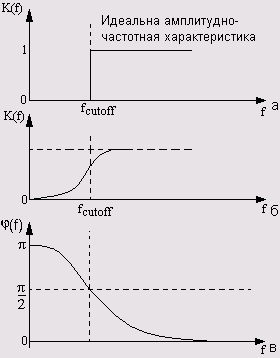
\includegraphics[width=0.4\textwidth]{pic-filter-01}}
\end{frame}

\begin{frame}
\centering{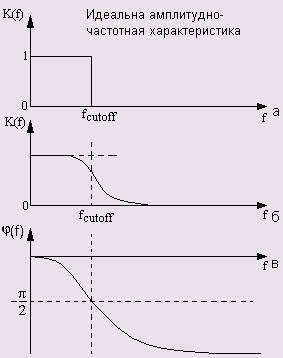
\includegraphics[width=0.4\textwidth]{pic-filter-02}}
\end{frame}

\begin{frame}
\emph{Крутизна спада} фильтра определяется как величина изменения коэффициента ослабления на частотах, отстоящих друг от друга на одну октаву (ед. изм.~--– дБ/октаву). Фильтр с крутизной 6 дБ на октаву называется фильтром первого порядка, 12 дБ на октаву~--– второго порядка и т.д.

~

Полоса пропускания полосно-пропускающих фильтров определяется как диапазон частот, в котором усиление находится в пределах 3 дБ от максимума. Полоса подавления режекторных фильтров определяется как диапазон частот, в котором ослабление находится в пределах 3 дБ от максимума.

~

Середина полосы пропускания называется \emph{центральной частотой}.

~

\emph{Коэффициент усиления} (\emph{ослабления}) полосно-пропускающих (режекторных) фильтров задает величину усиления (подавления) на центральной частоте.
\end{frame}

\begin{frame}
\centering{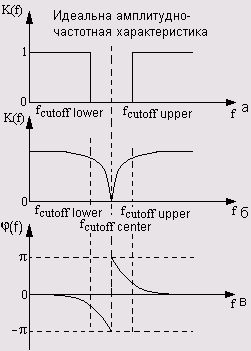
\includegraphics[width=0.4\textwidth]{pic-filter-03}}
\end{frame}

\begin{frame}
\centering{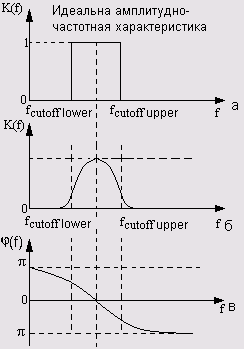
\includegraphics[width=0.4\textwidth]{pic-filter-04}}
\end{frame}

\begin{frame}
Часто вместо полосы пропускания используется понятие добротности (обозначается \emph{Q}), вычисляемое как отношение центральной частоты к ширине полосы пропускания. 

~

При $Q=15$ можно точно удалить синусоидальный сигнал постоянной частоты без заметного воздействия на окружающие частоты.

\centering{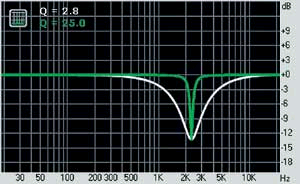
\includegraphics[width=0.4\textwidth]{pic-filter-05}}
\end{frame}

\begin{frame}
\emph{Фазо-частотная характеристика} фильтра показывает, как меняется фаза сигнала при фильтрации. Если фаза меняется на величину, пропорциональную частоте, то это соответствует простому сдвигу сигнала во времени, без изменения его формы. ФЧХ важна, так как сигнал, прошедший через фильтр без изменения амплитуды в полосе пропускания, может быть искажен по форме, если временное запаздывание при прохождении через фильтр не будет постоянным для разных частот.

~

Одинаковое время задержки соответствует линейной зависимости фазы от частоты. Для ФНЧ и ФВЧ зависимость фазы от частоты можно считать линейной лишь в окрестностях частот среза, а для полосового фильтра~--- в окрестностях центральной частоты.

~

Фильтрация звука в широкой полосе будет обязательно сопровождаться фазовыми искажениями, приводящими к изменению формы сигнала.
\end{frame}

\begin{frame}
Эквалайзеры представляют собой устройства, объединяющие в себе несколько фильтров, предназначенные для изменения спектральных свойств (тембра) обрабатываемого сигнала. Первоначально эквалайзер (\emph{equalizer}, \emph{EQ}) выполнял функции устройства, компенсирующего неравномерность того или иного участка тракта усиления и преобразования звукового сигнала.

~

Различают два вида эквалайзеров:
\begin{itemize}
  \item графический эквалайзер;
  \item параметрический эквалайзер.
\end{itemize}

~

\emph{Кроссовер}~--- устройство, которое разделяет входной сигнал на несколько выходных, причем каждый выходной сигнал содержит колебания только определенного диапазона частот.
\end{frame}

\end{document}
